\section{Vandermonde matrix}

For this exercise I needed to solve an equation containing a Vandermonde matrix using LU decomposition and Neville\'s algorithm.
Because I could copy all of the functions from the working classes, 
my code for those is similar to my sister\'s, Liz van der Kamp (s2135752). 
The only function not directly taken from my tutorial code is the one iterating on the LU solution to improve it, 
but the method for multiplying a matrix by a vector by doing np.sum(A*x, axis=1) I also took from my tutorial code in collaboration with Liz.

The code I wrote for this is:
\lstinputlisting{NUR_handin1Q2.py}

\subsection{a}
To read in the Vandermonde.txt file, I copied the example code provided in the Handin, 
then I generated the Vandermonde matrix and executed LU decomposition.
From the LU decomposition, I get the LU matrix, the solution for c, 
and an array of indexes which have saved which rowswaps I have done so I can reuse the LU matrix and my code later on without having to swap rows back.
Then, I get the interpolated result $y = \sum_j c_j x^j$ both for my 1000 x points and my initial x$_i$ so I can compare to the initial data points, 
and I plot the results in Fig. \ref{fig:fig1}.
The resulting solution for for c is:
\lstinputlisting{NUR1_c_sol1.txt}

\begin{figure}[h!]
  \centering
  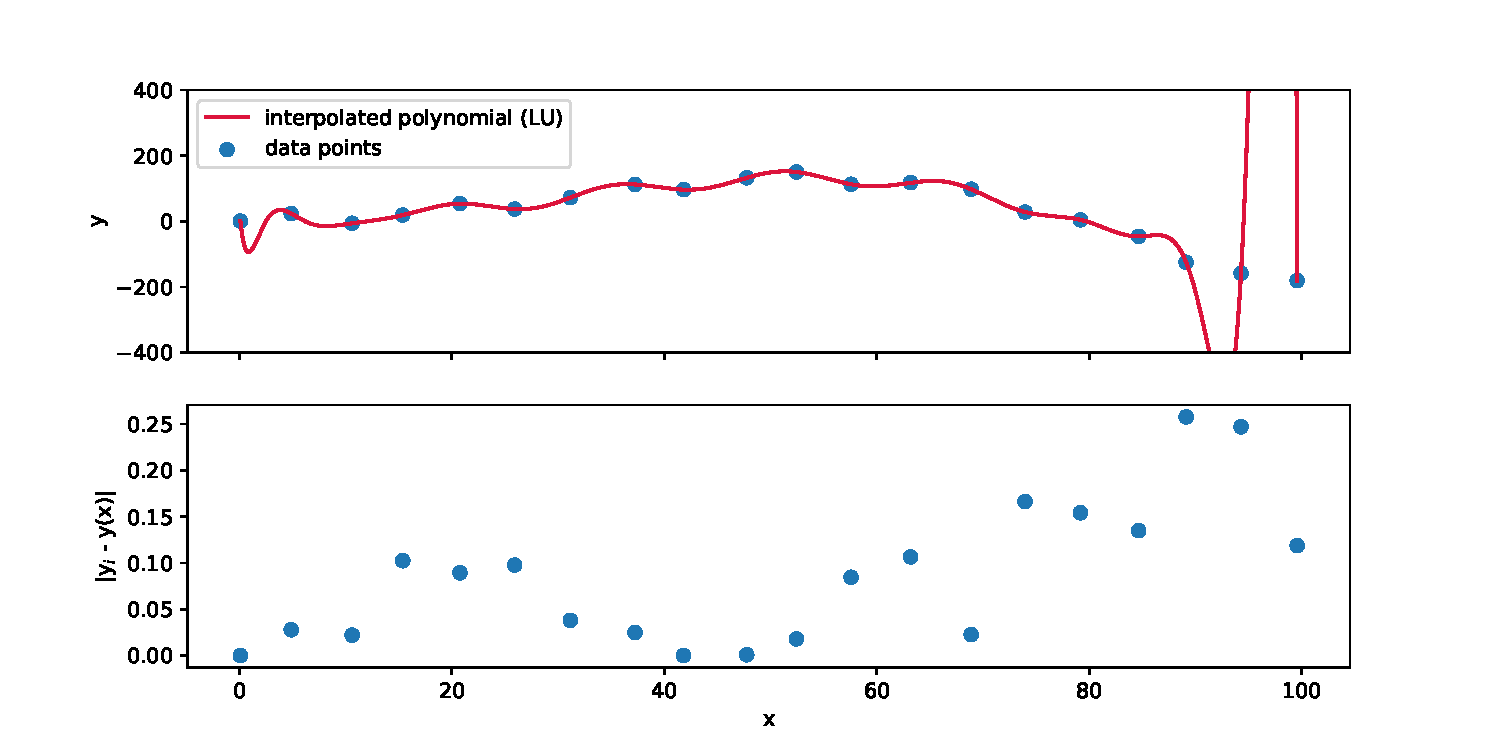
\includegraphics[width=0.9\linewidth]{NUR1_Q2_plot1.pdf}
  \caption{Plot corresponding to exercise 2a. The top plot shows the data points 
  and the interpolated 19th degree polynomial given by the LU decomposition. The bottom plot shows the absolute difference between
  the data points and the result from the LU decomposition.}
  \label{fig:fig1}
\end{figure} 

\subsection{b}
Using the function for Neville\'s algorithm I made during the tutorial (together with Liz), I calculate the interpolated 19th degree polynomial for my 1000 x points and my initial x$_i$ so I can compare to the initial data points again, and I plot the results in comparison to my result in (a) in Fig. \ref{fig:fig2}.

\begin{figure}[h!]
  \centering
  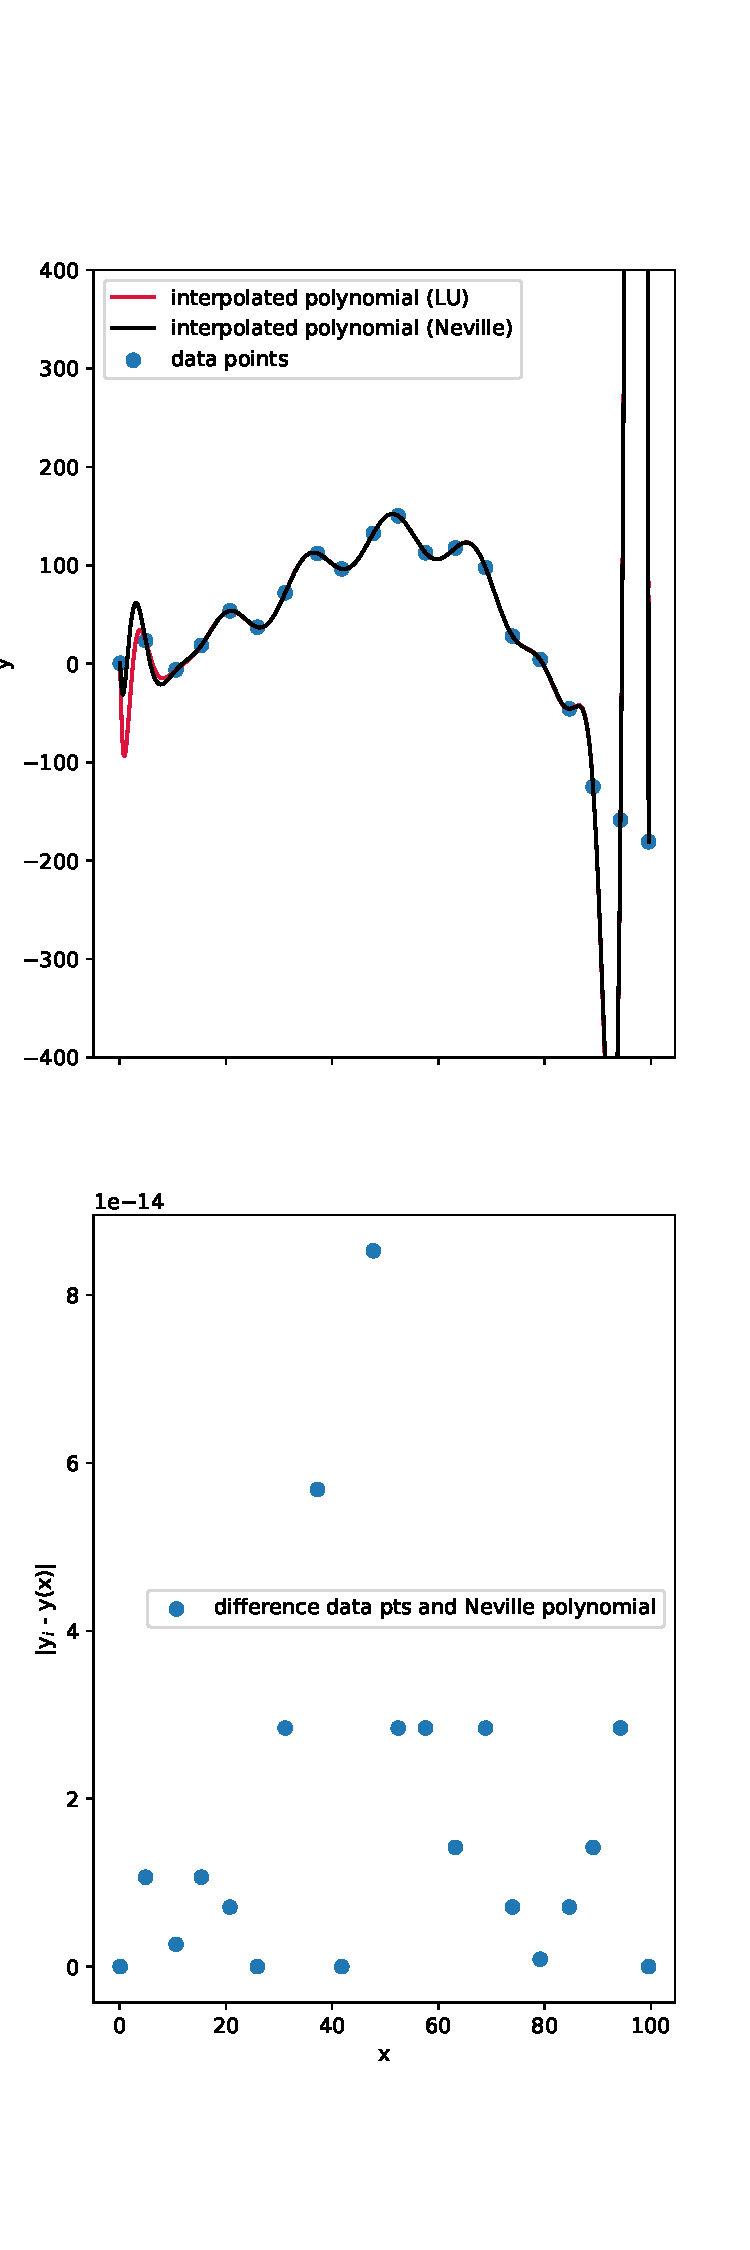
\includegraphics[width=0.9\linewidth]{NUR1_Q2_plot2.pdf}
  \caption{Plot corresponding to exercise 2b. The top plot shows the data points, the interpolated 19th degree polynomial given by the LU decomposition (red), and the interpolated 19th degree polynomial from Neville\'s algorithm (black). The bottom plot shows the absolute difference between
  the data points and the result from Neville\'s algorithm.}
  \label{fig:fig2}
\end{figure} 

You can see that the first bit of Neville\'s algorithm and the LU decomposition do not match (on the range x~0-20), and that the absolute difference between the data and the interpolation is bigger for LU decomposition than for Neville\'s algorithm. 
This makes sense because Neville\'s algorithm already improves it by iterating over the solution 19 times for a 19th degree polynomial, while LU decomposition does only 1 iteration. 


\subsection{c}
To improve the result from (a), I take the part of my LU decomposition code with uses the LU matrix to solve for the answer, and make a function which takes the matrix M, the LU decomposition of M, x and b such that Mx = b, the index array containing which rows were swapped, and the number of iterations.
Then, the function takes del\_b = Mx - b = del\_x, and solves to get del\_x, which I substract from our initial x to get a new estimate, which I then use to get a new del_b and del\_x to improve the solution again, and that repeats the number of times given by "iter". 
The improved solution for c is: 
\lstinputlisting{NUR1_c_sol10.txt}
I plot this result compared to the 1 time iterated solution from (a) and plot the absolute difference again, see Fig. \ref{fig:fig3}. You can see that the absolute difference has reduced a lot compared to (a), except for at the end points.

\begin{figure}[h!]
  \centering
  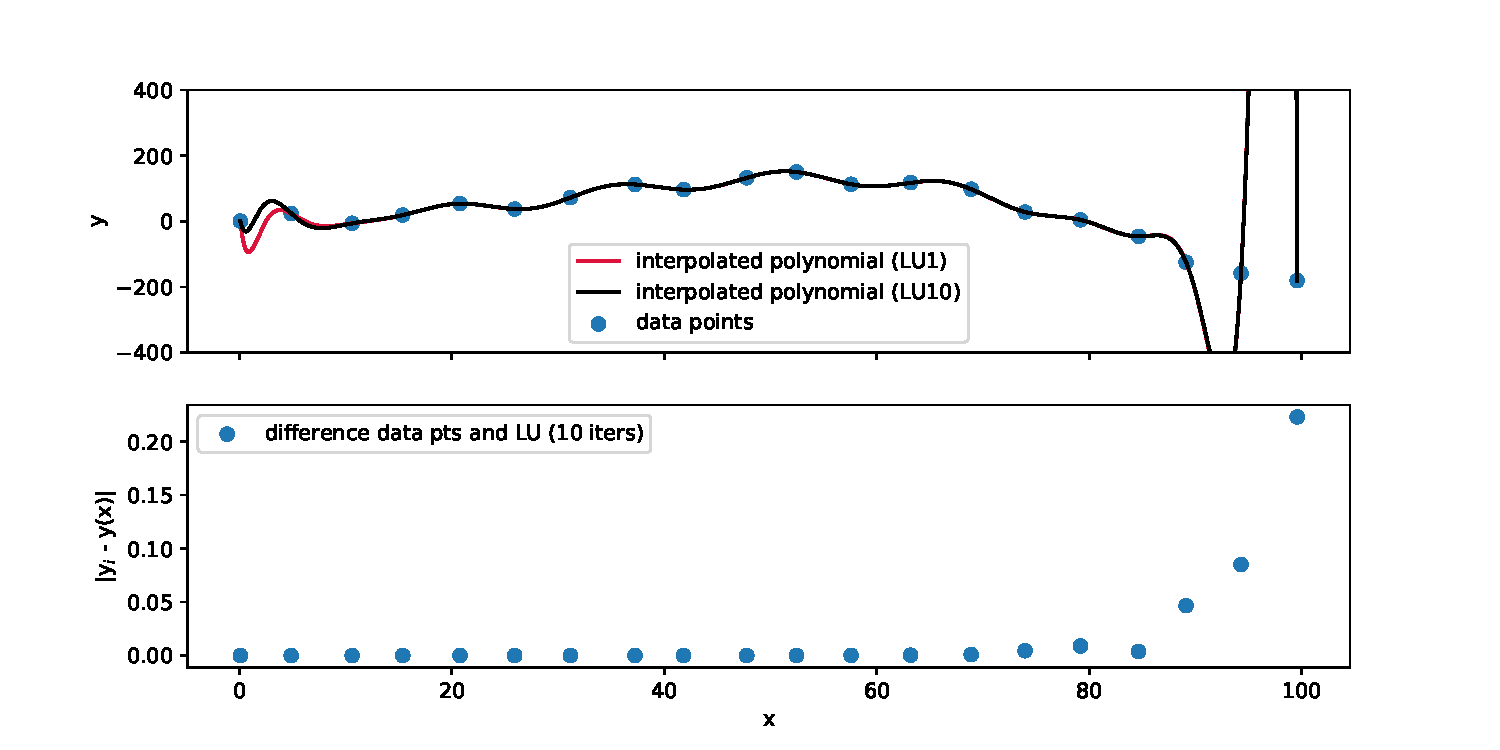
\includegraphics[width=0.9\linewidth]{NUR1_Q2_plot3.pdf}
  \caption{Plot corresponding to exercise 2c. The top plot shows the data points, the interpolated 19th degree polynomial given by the LU decomposition with 1 iteration (red), and the interpolated 19th degree polynomial given by the LU decomposition with 10 iterations (black). The bottom plot shows the absolute difference between
  the data points and the result from LU decomposition with 10 iterations.}
  \label{fig:fig3}
\end{figure} 


\subsection{d}
I use timeit and a for loop to run the functions for (a), (b), and (c) 20 times and return the average time it took. The results are, for (a), (b), and (c) respectively (in seconds):
\lstinputlisting{NUR1_c_sol10.txt, NUR1_Q2_avertimes.txt}
As you can see, the LU decomposition and improving it 10x take about the same time, which is both more than 10x faster than Neville's algorithm, so doing the LU decomposition + improvement is most efficient because for Neville you have to do bisection for every point and then interpolate and iterate many times, which is slow if you want to do it for many points
LU decomposition just uses 1 matrix you have to calculate once and thus improving the solution is efficient because you can use the same matrix every time, and you only have to solve it.
From the plots, Neville\'s algorithm yields the most accurate solution because it already iterates a lot of times to more precisely calculate the polynomial, and it combines more and more accurate estimates to get a better solution, while LU iteration does not combine anything, it just uses the error estimate to get a better solution. 
